% questions.tex —— 1993 年·新科目组·理科 · 题目内容片段（无答案）
% 由 tools/generate_projects.py 依来源总账自 1993/1993_数学真题_新科目组理_试题.md 生成，勿手改（改源 MD 后重跑）


\gkpart{数学}

\begin{gktip}
\textbf{来源说明}：依据固定来源 PDF 的原生文字层逐题转录，并对照 400 dpi 页面渲染逐题核对。源为 \textbf{XeTeX 重排件（非扫描）}——全矢量、文字层可读、嵌入 LM／CM 系与 STSong／STHeiti 字体。单页 A3 横向三栏（页面 1190.55×841.89 pt），页脚仅印印刷页码 \textbf{45}；\textbf{源页无大题标题}，题号 1–28 连续；\textbf{无答案页}。

\textbf{标点与字样约定}：① 题号源内为半角句点，本库统一作全角「．」；② 源内句末为实心点「．」，按全库约定归一为「。」，其余中文标点归一全角；③ 选项标号源为半角「(A)」，排印统一作全角「（A）」；④ 分数按源竖排真分式，排印用 \(\dfrac{a}{b}\)；⑤ 虚数单位 \(\mathrm{i}\) 为正体。

\textbf{存疑与登记}（源内异常照录，不推测补正）：第 21 题 \(f^{-1}(0)\) 记号未说明约定；第 28 题未声明 \(\arg\) 的值域。两题照录原样，判定见答案卷。

\textbf{图示}：第 23 题折叠正方形示意（两幅：折叠前的正方形 \(ABCD\) 与折痕 \(DE\)、\(CE\)；折叠后 \(A\)、\(B\) 重合于 \(P\)），按源 PDF 内容流逐路径重绘（线宽 0.398pt、虚线 [2.989 2.989]，标签取源文本中心），不按比例。
\end{gktip}

\begin{question}
\gkti{1}函数 $f(x)=\sin x+\cos x$ 的最小正周期是\mbox{（　　）}。

（A）$2\pi$　　（B）$2\sqrt2\pi$　　（C）$\pi$　　（D）$\dfrac\pi4$

\end{question}
\begin{question}
\gkti{2}如果双曲线的焦距为 $6$，两条准线间的距离为 $4$，那么该双曲线的离心率为\mbox{（　　）}。

（A）$\dfrac32$　　（B）$\dfrac{\sqrt3}{2}$　　（C）$\dfrac{\sqrt6}{2}$　　（D）$2$

\end{question}
\begin{question}
\gkti{3}和直线 $3x-4y+5=0$ 关于 $x$ 轴对称的直线的方程为\mbox{（　　）}。

（A）$3x+4y-5=0$　　（B）$3x+4y+5=0$

（C）$-3x+4y-5=0$　　（D）$-3x+4y+5=0$

\end{question}
\begin{question}
\gkti{4}极坐标方程 $\rho=\dfrac4{3-5\cos\theta}$ 所表示的曲线是\mbox{（　　）}。

（A）焦点到准线距离为 $\dfrac45$ 的椭圆

（B）焦点到准线距离为 $\dfrac45$ 的双曲线右支

（C）焦点到准线距离为 $\dfrac43$ 的椭圆

（D）焦点到准线距离为 $\dfrac43$ 的双曲线右支

\end{question}
\begin{question}
\gkti{5}$y=x^{3/5}$ 在 $[-1,1]$ 上是\mbox{（　　）}。

（A）增函数且是奇函数　　（B）增函数且是偶函数

（C）减函数且是奇函数　　（D）减函数且是偶函数

\end{question}
\begin{question}
\gkti{6}$\displaystyle\lim_{n\to\infty}\dfrac{5n^2-1}{2n^2-n+5}$ 的值为\mbox{（　　）}。

（A）$-\dfrac15$　　（B）$-\dfrac52$　　（C）$\dfrac15$　　（D）$\dfrac52$

\end{question}
\begin{question}
\gkti{7}集合
$M=\left\{x\mid x=\dfrac{k\pi}{2}+\dfrac\pi4,\ k\in\mathbb Z\right\}$，
$N=\left\{x\mid x=\dfrac{k\pi}{4}+\dfrac\pi2,\ k\in\mathbb Z\right\}$，
则\mbox{（　　）}。

（A）$M=N$　　（B）$M\supseteq N$　　（C）$M\subseteq N$　　（D）$M\cap N=\varnothing$

\end{question}
\begin{question}
\gkti{8}$\sin20^\circ\cos70^\circ+\sin10^\circ\sin50^\circ$ 的值是\mbox{（　　）}。

（A）$\dfrac14$　　（B）$\dfrac{\sqrt3}{2}$　　（C）$\dfrac12$　　（D）$\dfrac{\sqrt3}{4}$

\end{question}
\begin{question}
\gkti{9}参数方程
\nopagebreak[4]
\[
\begin{cases}
x=\cos\dfrac\theta2+\sin\dfrac\theta2,\\
y=\dfrac12(1+\sin\theta),
\end{cases}\quad(0<\theta<2\pi)
\]
表示\mbox{（　　）}。

（A）双曲线的一支，这支过点 $\left(1,\dfrac12\right)$

（B）抛物线的一部分，这部分过点 $\left(1,\dfrac12\right)$

（C）双曲线的一支，这支过点 $\left(-1,\dfrac12\right)$

（D）抛物线的一部分，这部分过点 $\left(-1,\dfrac12\right)$

\end{question}
\begin{question}
\gkti{10}若 $a\text{、}b$ 是任意实数，且 $a>b$，则\mbox{（　　）}。

（A）$a^2>b^2$　　（B）$\dfrac ba<1$

（C）$\lg(a-b)>0$　　（D）$\left(\dfrac12\right)^a<\left(\dfrac12\right)^b$

\end{question}
\begin{question}
\gkti{11}一动圆与两圆 $x^2+y^2=1$ 和 $x^2+y^2-8x+12=0$ 都外切，则动圆圆心轨迹为\mbox{（　　）}。

（A）圆　　（B）椭圆　　（C）双曲线的一支　　（D）抛物线

\end{question}
\begin{question}
\gkti{12}圆柱轴截面的周长 $l$ 为定值，那么圆柱体积的最大值是\mbox{（　　）}。

（A）$\left(\dfrac l6\right)^3\pi$　　（B）$\dfrac19\left(\dfrac l2\right)^3\pi$

（C）$\left(\dfrac l4\right)^3\pi$　　（D）$2\left(\dfrac l4\right)^3\pi$

\end{question}
\begin{question}
\gkti{13}$(\sqrt{x}+1)^4(x-1)^5$ 展开式中 $x^4$ 的系数为\mbox{（　　）}。

（A）$-40$　　（B）$10$　　（C）$40$　　（D）$45$

\end{question}
\begin{question}
\gkti{14}直角梯形的一个内角为 $45^\circ$，下底长为上底长的 $\dfrac32$，这个梯形绕下底所在的直线旋转一周所成的旋转体的全面积为 $(5+\sqrt2)\pi$，则旋转体的体积为\mbox{（　　）}。

（A）$2\pi$　　（B）$\dfrac{4+\sqrt2}{3}\pi$

（C）$\dfrac{5+\sqrt2}{3}\pi$　　（D）$\dfrac73\pi$

\end{question}
\begin{question}
\gkti{15}已知 $a_1,a_2,\ldots,a_8$ 为各项都大于零的等比数列，公比 $q\ne1$，则\mbox{（　　）}。

（A）$a_1+a_8>a_4+a_5$

（B）$a_1+a_8<a_4+a_5$

（C）$a_1+a_8=a_4+a_5$

（D）$a_1+a_8$ 和 $a_4+a_5$ 的大小关系不能由已知条件确定

\end{question}
\begin{question}
\gkti{16}设有如下三个命题：

甲：相交两直线 $l,m$ 都在平面 $\alpha$ 内，并且都不在平面 $\beta$ 内。

乙：$l,m$ 之中至少有一条与 $\beta$ 相交。

丙：$\alpha$ 与 $\beta$ 相交。

当甲成立时\mbox{（　　）}。

（A）乙是丙的充分而不必要的条件

（B）乙是丙的必要而不充分的条件

（C）乙是丙的充分且必要的条件

（D）乙既不是丙的充分条件又不是丙的必要条件

\end{question}
\begin{question}
\gkti{17}将数字 $1,2,3,4$ 填入标号为 $1,2,3,4$ 的四个方格里，每格填一个数字，则每个方格的标号与所填的数字均不相同的填法有\mbox{（　　）}。

（A）$6$ 种　　（B）$9$ 种　　（C）$11$ 种　　（D）$23$ 种

\end{question}
\begin{question}
\gkti{18}$\displaystyle\sin\left(\arccos\dfrac12+\arccos\dfrac13\right)=$\underline{\qquad\qquad}。

\end{question}
\begin{question}
\gkti{19}若双曲线 $\dfrac{x^2}{9k^2}-\dfrac{y^2}{4k^2}=1$ 与圆 $x^2+y^2=1$ 没有公共点，则实数 $k$ 的取值范围为\underline{\qquad\qquad}。

\end{question}
\begin{question}
\gkti{20}从 $1,2,\ldots,10$ 这十个数中取出四个数，使它们的和为奇数，共有\underline{\qquad\qquad}种取法（用数字作答）。

\end{question}
\begin{question}
\gkti{21}设 $f(x)=4^x-2^{x+1}$，则 $f^{-1}(0)=$\underline{\qquad\qquad}。

\end{question}
\begin{question}
\gkti{22}建造一个容积为 $8\,\mathrm{m}^3$、深为 $2\,\mathrm m$ 的长方体无盖水池。如果池底和池壁的造价每平方米分别为 $120$ 元和 $80$ 元，那么水池的最低总造价为\underline{\qquad\qquad}元。

\Needspace{0.4\textheight}
\end{question}
\begin{question}
\gkti{23}如图，$ABCD$ 是正方形，$E$ 是 $AB$ 的中点。如将 $\triangle DAE$ 和 $\triangle CBE$ 分别沿虚线 $DE$ 和 $CE$ 折起，使 $AE$ 与 $BE$ 重合，记 $A$ 与 $B$ 重合的点为 $P$，则面 $PCD$ 与面 $ECD$ 所成的二面角为\underline{\qquad\qquad}度。
\nopagebreak[4]
\begin{center}% 1993_新科目组_理科/figures/f1993_new_science_q23_fold.tex — 1993 年·新科目组·理科 第 23 题（折叠正方形示意）
%
% 【来源】`.work/phase4-b17/source/1993新科目组理.pdf`（SHA-256 14297950237f422e346d8c8a60ba0a9bb18d2ac4bcb69de4dabcb0ae2e83bd2d），第 1 页；
%   内容流 `q 1 0 0 1 901.783 516.913 cm` 段逐路径照录，
%   解析脚本 `.work/phase4-b17/probe/pdfparse_full.py`。
%
% 【坐标口径】源 PDF 用户空间（原点左下、y 向上）。本图本地坐标
%   (x,y) = (x_page − 901.783, y_page − 516.913)，1 单位 = 1 TeX pt。
%   线宽 0.398pt；虚线 [2.989 2.989] 0 d。
%
% 元素计数：实线 10 段（正方体四边、折叠后 D′C′/D′E′/C′E′/PE/PD′/PC′）+ 虚线 2 段（DE、CE）+ 9 个标签。
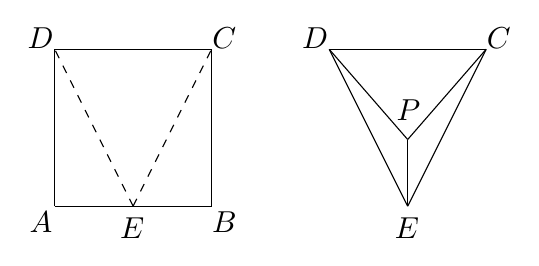
\begin{tikzpicture}[x=1pt, y=1pt,
    every node/.style={inner sep=0pt, font=\fontsize{10.5pt}{12.6pt}\selectfont}]
  \draw[line width=0.398pt] (0.000,0.000) -- (56.694,0.000);
  \draw[line width=0.398pt] (56.694,56.694) -- (56.694,0.000);
  \draw[line width=0.398pt] (56.694,56.694) -- (0.000,56.694);
  \draw[line width=0.398pt] (0.000,0.000) -- (0.000,56.694);
  \draw[line width=0.398pt] (99.214,56.694) -- (127.561,0.000);
  \draw[line width=0.398pt] (155.907,56.694) -- (127.561,0.000);
  \draw[line width=0.398pt] (155.907,56.694) -- (99.214,56.694);
  \draw[line width=0.398pt] (127.561,24.095) -- (127.561,0.000);
  \draw[line width=0.398pt] (127.561,24.095) -- (99.214,56.694);
  \draw[line width=0.398pt] (127.561,24.095) -- (155.907,56.694);
  % 虚线：正方形内 DE、CE（折痕）
  \draw[line width=0.398pt, dash pattern=on 2.989pt off 2.989pt] (28.347,0.000) -- (0.000,56.694);
  \draw[line width=0.398pt, dash pattern=on 2.989pt off 2.989pt] (28.347,0.000) -- (56.694,56.694);
  \node[anchor=center] at (-5.070,60.770) {$D$};
  \node[anchor=center] at (61.250,60.770) {$C$};
  \node[anchor=center] at (-4.930,-5.780) {$A$};
  \node[anchor=center] at (28.050,-7.820) {$E$};
  \node[anchor=center] at (61.360,-5.780) {$B$};
  \node[anchor=center] at (94.140,60.770) {$D$};
  \node[anchor=center] at (160.470,60.770) {$C$};
  \node[anchor=center] at (127.830,34.700) {$P$};  % 相对源中心上移 2.49pt、右移 1.0pt，避开 D–P 边
  \node[anchor=center] at (127.260,-7.820) {$E$};
\end{tikzpicture}
%
% 【自验结果】探针：坐标逐点照录内容流；与 400 dpi 渲染并排比对（标签位置取 pdftotext -bbox 中心）。
\end{center}
\nopagebreak[4]
\end{question}
\begin{question}
\gkti{24}已知 $f(x)=\log_a\dfrac{1+x}{1-x}\ (a>0,\ a\ne1)$。

(1) 求 $f(x)$ 的定义域；

(2) 判断 $f(x)$ 的奇偶性并予以证明；

(3) 求使 $f(x)>0$ 的 $x$ 取值范围。

\end{question}
\begin{question}
\gkti{25}已知数列
$\dfrac{8\cdot1}{1^2\cdot3^2},\ \dfrac{8\cdot2}{3^2\cdot5^2},\ \ldots,\ \dfrac{8n}{(2n-1)^2(2n+1)^2},\ \ldots$，$S_n$ 为其前 $n$ 项和。
计算得 $S_1=\dfrac89,\ S_2=\dfrac{24}{25},\ S_3=\dfrac{48}{49},\ S_4=\dfrac{80}{81}$。观察上述结果，推测出计算 $S_n$ 的公式，并用数学归纳法加以证明。

\end{question}
\begin{question}
\gkti{26}已知：平面 $\alpha\cap$ 平面 $\beta=$ 直线 $a$。$\alpha,\beta$ 同垂直于平面 $\gamma$，又同平行于直线 $b$。求证：(1) $a\perp\gamma$；(2) $b\perp\gamma$。

\end{question}
\begin{question}
\gkti{27}在面积为 $1$ 的 $\triangle PMN$ 中，$\tan\angle PMN=\dfrac12,\ \tan\angle MNP=-2$。建立适当的坐标系，求以 $M,N$ 为焦点且过点 $P$ 的椭圆方程。

\end{question}
\begin{question}
\gkti{28}\looseness=-1 设复数 $z=\cos\theta+i\sin\theta\ (0<\theta<\pi)$，
$\omega=\dfrac{1-(\overline z)^4}{1+z^4}$，并且 $|\omega|=\dfrac{\sqrt3}{3}$，$\arg\omega<\dfrac\pi2$，求 $\theta$。

\end{question}